\paragraph{Naming the unknown is what works} When we let the planner say ``none of the above'', it found \SimTprP\ of the never-seen event types at a 5\% false-alarm rate. The usual alternative, a threshold on how uncertain a closed-world planner is, found only \SimTprBthree\ (Fig.~\ref{fig:rocsim}). Without that extra option, closed-world information gain was confidently wrong on \SimCwWhBthreeAll\ of the unknown events, against \SimCwWhPAll\ for our planner P. It paid nothing for this on ordinary events, and kept the same accuracy on the known classes (\SimAccModPAll). We then checked whether P's gain comes from where it chooses to measure. It does not, since an uncertainty threshold computed on P's own measurements still reached an AUROC of only \SimAucPown, against \SimAucP\ for $P(h_0)$. So the gain comes from having a name for the unknown, not from clever measurement.

\begin{figure}[!tbp]
\centering
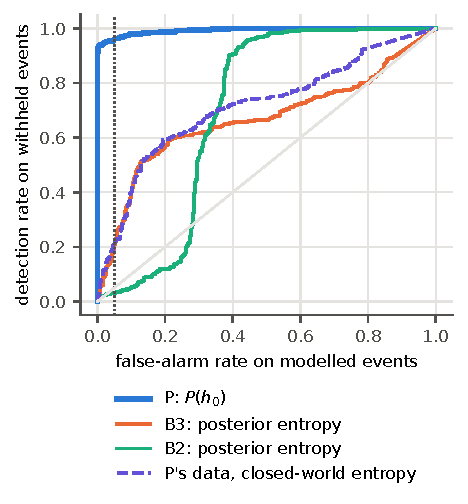
\includegraphics[width=\columnwidth]{generated/figures/fig3_roc_sim.pdf}
\caption{Simulation. How well each method separates never-seen event types from known ones. The dotted line marks the 5\% false-alarm point we fixed in advance.}
\label{fig:rocsim}
\end{figure}

\paragraph{It is not the fastest} We expected P to identify known events sooner than every baseline, and it did not. A cheap rule that measures where classifiers disagree got there first on the events it could identify (median \SimTtiBtwo\ against \SimTtiP), but it gave up on many of them, identifying only \SimIdBtwo\ of events against \SimIdP\ for P (Fig.~\ref{fig:tti}).

\begin{figure}[!tbp]
\centering
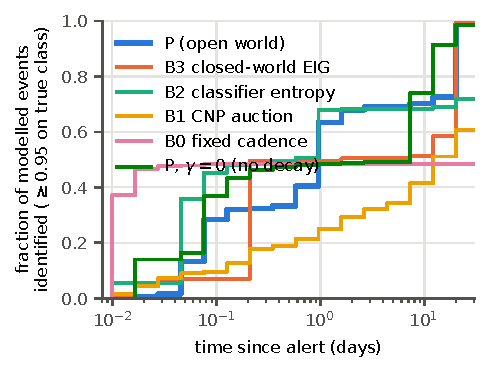
\includegraphics[width=\columnwidth]{generated/figures/fig1_tti.pdf}
\caption{Simulation. Share of known events identified (posterior on the true class at least 0.95) against time since the alert. The disagreement rule B2 is quickest on the events it can identify, while P identifies almost all of them, a little later.}
\label{fig:tti}
\end{figure}

\paragraph{Urgency helps fast events, but not all of them} The decay term is meant to make the planner measure fast events before they fade. It did recover more information on kilonovae (\SimDeltaKilonova) and shock cooling (\SimDeltaShock) than on the slow GRB afterglow, but for the fastest class, the M-dwarf flare, it lost information (\SimDeltaFlare; Fig.~\ref{fig:decay}), and it reversed under model error. Its clearest benefit was indirect. Without it, the planner spent its measurements too early (\SimObsAllNoDecay\ instead of \SimObsAllP), which left $h_0$ too little data and raised confident errors on unknowns to \SimCwWhNoDecayAll. The term built to test $h_0$ directly ($\beta$) changed nothing we could measure.

\begin{figure}[!tbp]
\centering
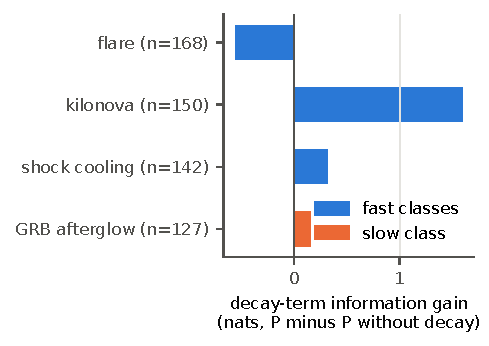
\includegraphics[width=\columnwidth]{generated/figures/fig2_decay.pdf}
\caption{Simulation. Information about each event's brightness gained from the decay term (P minus P without it). It helps kilonovae and shock cooling, does little for the slow class, and hurts flares.}
\label{fig:decay}
\end{figure}

\begin{table*}[!tbp]
\centering\scriptsize
\caption{Simulation test results (1000 events per scenario). Acc.\ mod.: accuracy on modelled events (\%). CW: confident-wrong rate (\%) on unmodelled (withheld) and modelled events. $\bar n_{\rm obs}$: measurements used, out of 5. Log score: mean log probability of the true outcome (closed-world strategies cannot express ``withheld'', so they are floored at $10^{-6}$).}
\label{tab:sim}
\begin{tabular}{llrrrrr}
\toprule
Scenario & Strategy & Acc.\ mod. & CW unmod. & CW mod. & $\bar n_{\rm obs}$ & log score \\
\midrule
Nominal & P (open world) & 100 & 6 & 0 & 4.2 & -0.19 \\
 & B3 closed-world EIG & 100 & 97 & 0 & 2.8 & -5.71 \\
 & B2 classifier entropy & 88 & 69 & 0 & 4.9 & -5.82 \\
 & B1 CNP auction & 80 & 75 & 0 & 3.2 & -5.92 \\
 & B0 fixed cadence & 79 & 1 & 0 & 5.0 & -5.92 \\
 & P, $\gamma=0$ (no decay) & 99 & 31 & 0 & 3.6 & -0.87 \\
 & P, $\beta=0$ (no adequacy) & 100 & 6 & 0 & 4.3 & -0.20 \\
\midrule
Crowding & P (open world) & 99 & 14 & 0 & 4.0 & -0.43 \\
 & B3 closed-world EIG & 100 & 94 & 0 & 3.0 & -5.82 \\
 & B2 classifier entropy & 94 & 80 & 0 & 4.8 & -5.88 \\
 & B1 CNP auction & 86 & 71 & 0 & 3.1 & -5.97 \\
 & B0 fixed cadence & 76 & 1 & 0 & 5.0 & -6.03 \\
 & P, $\gamma=0$ (no decay) & 100 & 31 & 0 & 3.4 & -0.96 \\
 & P, $\beta=0$ (no adequacy) & 99 & 14 & 0 & 4.1 & -0.43 \\
\midrule
Model error & P (open world) & 87 & 21 & 8 & 3.9 & -1.21 \\
 & B3 closed-world EIG & 99 & 96 & 1 & 2.9 & -6.11 \\
 & B2 classifier entropy & 81 & 29 & 4 & 5.0 & -6.32 \\
 & B1 CNP auction & 82 & 72 & 1 & 3.2 & -6.29 \\
 & B0 fixed cadence & 77 & 1 & 0 & 5.0 & -6.25 \\
 & P, $\gamma=0$ (no decay) & 93 & 26 & 6 & 3.4 & -1.32 \\
 & P, $\beta=0$ (no adequacy) & 86 & 21 & 8 & 3.9 & -1.21 \\
\bottomrule
\end{tabular}

\end{table*}
